\chapter[The Shell]{}

\section{Getting around}

Once you have a shell, you'll want to be able to move around the system. 
This chapter will outline how to look around the system that you're on.

\subsection{Where am I?}
The first thing that you need to do to go somewhere is find where you are!  
The {\tt pwd(1)} command will give the path to the folder that you are currently in.  
Literally, it give you the {\tt P}resent {\tt W}orking {\tt D}irectory.   
What does that this look like?
{\\
\tt \# pwd\\
/home/john\\
\#\\
}
On the machine we are on, we are in John's home folder.

Great, now that we know where we are, should look to see what is all in the folder we are in. To do this, we use the {\tt ls(1)} command. {\tt ls} stands for list or listing -- it will give you a listing of all the files and folders in the current folder.

What does this look like?
{\tt \begin{verbatim}\\
\# ls\\
oldhome\ \ \ \ \ \ Desktop\ \ \ \ \ \ Mail\ \ \ \ \ \ \ \ \ public\_html\\
check\ \ \ \ \ \ \ \ Documents\ \ \ \ temp\\
\# \\
\end{verbatim}
}

Now that we have a listing of all the files and folders, we have to figure out which ones are files, and which ones are folders.  Sometimes it's not completely clear from the name which are which.

For this we use the command {\tt ls -l}, which is the same command uses what's called a Command Line Switch.  Command line switches are used
to change the way a command functions.  In this case, the {\tt -l} switch means ``long", and will print out a more detailed listing of the items in the current directory.

% [TODO: talk about the file extention for the excecutable?  Link it to where it's discussed]

{\tt 
\begin{verbatim}
# ls -l
drwxr-xr-x   2 john student     4096 Apr 11  2005 oldhome
drwxr-xr-x   2 john student     4096 Jan 10  2008 check
drwxr-xr-x   2 john student     4096 Jan  9  2007 Desktop
drwxr-xr-x   2 john student     4096 Nov 28  2005 Documents
drwx------   3 john student     4096 Nov 24  2005 Mail
drwxr--r--   2 john student     4096 Jul 22  2009 public_html
-rw-------   1 john student     5543 Aug  5 15:16 temp
#



\end{verbatim}
}

When we do this, we can see a lot about the items in the directory we are in. Each line has the same format.
{\tt
\begin{verbatim}
\[FileAccessRights\] \[hard link count\] \[owner\] \[group\]    \[size\]  \[modification date\]  \[name\]
\end{verbatim}
}

The first section is the file access rights.  This will tell you who can control this file, and how.  This is described in the {\tt chmod} 
section, so for now just note you can see it this way.  The think that we are interested in is 
the first letter of the line.  If the line starts with a {\tt d}, that item is a directory.  If it starts with a {\tt -} it
is a file.  From the above example you can see that {\tt public\_html} is a folder, and {\tt temp} is a file.

The hard link count section we will leave a mystery, since most people ignore this field.

One interesting thing to note is that there are hidden files in some directories, most notably, your home folder.

% TODO - this list is not pretty.
%  either put it on it's own page
%  or clean it up.
% at least make sure it fits on one page? Create an image out of it which is
% a page long?
{\tt
\begin{verbatim}
# ls -al
drwx--x--x  34 john student     4096 Aug  5 15:16 .
drwxr-xr-x 2779 root     root      253952 Aug  4 19:38 ..
drwxr-xr-x   2 john student     4096 Oct 29  2004 .acrobat
-rw-r--r--   1 john student      237 Apr 25  2005 .acrosrch
drwx------   2 john student     4096 Apr  5  2005 .adobe
-rw-------   1 john student      878 Feb  5  2010 .bash_history
-rwx------   1 john student      789 Sep  8  2003 .cshrc
drwxr-xr-x   2 john student     4096 Apr 11  2005 .desktop
-rw-------   1 john student       26 May  4  2006 .dmrc
-rw-r--r--   1 john student        0 Jan 10  2007 .fonts.cache-1
drwx------   4 john student     4096 Feb  2  2007 .gconf
drwx------   2 john student     4096 Feb  2  2007 .gconfd
drwx------   6 john student     4096 Apr 11  2005 .gnome
drwxr-xr-x   2 john student     4096 Jan  9  2007 .gnome-desktop
drwx------   8 john student     4096 Feb  2  2007 .gnome2
drwx------   5 john netscape    4096 Apr 11  2005 .netscape

[snip]

-rw-------   1 john student      269 Jan  9  2007 .recently-used
-rw-------   1 john student      497 May  4  2006 .rhn-applet.conf
-rw-r--r--   1 john student     1111 Mar  3  2005 .smc.properties
-rw-------   1 john student      733 Apr  6  2005 .TTauthority
drwx------   2 john student     4096 Apr  6  2005 .vnc
-rw-------   1 john student     3519 Feb  2  2007 .Xauthority
-rw-------   1 john student     5543 Aug  5 15:16 temp

[snip]
\end{verbatim}
}

Hidden files are prefixed with a period, which is effective and simple.  
On Unix-based operating systems such as Ubuntu and Mac OS you'll find 
there is a lot of hidden files.  This is because applications store 
preferences here for later use.  Applications
might store things like use names, recently used files or where you like 
the window to appear (assuming you have a windowing environment).
The machine in the example runs Gnome, which is a windowing environment, and it has left many hidden files for it to use.

\subsection{Moving Around}
Now that we know where we are, we need to be able to get around, or {\tt cd(1)} {\tt C}hange {\tt D}irectories.
We can {\tt cd} into any directory we have access to quite easily.
{\tt \begin{verbatim}
# /home/john
# cd Desktop
# pwd
/home/john/Desktop
#
\end{verbatim}
}
It's as easy as that! We knew that there was a folder named `Desktop' from the {\tt ls} 
we did, so we moved into that folder, as shown by {\tt pwd}.

It's quite easy to move into a folder, but now how do new back up to the 
previous, or parent folder? Take a look at the {\tt ls -a} output. 
{\tt \begin{verbatim}
# ls -al
drwxr-xr-x  12 john student     408 25 May 10:47 .
drwxr-xr-x  83 john student    2822  5 Aug 09:57 ..
\end{verbatim}
}

{\tt .} and {\tt ..} are two important characters in the shell environment.  A single period `.' means `this directory'. Two periods `..' means parent directory.

So, if we want to change to the parent directory we type {\tt cd ..}, which literally means `change directory to parent'.
{\tt \begin{verbatim}
# pwd
/home/john/Desktop
# cd ..
#
# pwd
/home/john
#
\end{verbatim}
}

We can also move up two directories up using close to the same command. Lots
 of people get this command wrong when they're first thinking about it.
{\tt \begin{verbatim}
# cd ..     # Goes to parent
# cd ....   # Must go two levels up? WRONG!

# cd ../..  # this is the command you want.
\end{verbatim}
}
% TODO - too strong?

What the command literally does is changes directory to the parent, 
then finds the `..' file in that directory, which is that directory's parent.

{\tt ls} can use the same path notation.  If we wanted to {\tt ls} the parent directory we 
could run this command:
{\tt \begin{verbatim}
# pwd
/home/john/Desktop/Videos
# ls ..
MyStuff       Videos        
#
\end{verbatim}
}

One other special characters that is useful when using {\tt cd} is the tilde ($\sim$). Tilde means `my home'.
{\tt \\    %didn't use 'verbatim' here to get the tilde to work.
\# pwd \\
/usr/local/bin \\
\# cd $\sim$ \\
\# pwd \\
/home/john \\
\# \\

}
 
 
And you can even do things like this, if you want, making complicated moves
around your filesystem.
{\tt \\
\# pwd \\
/usr/local/bin \\
\# cd $\sim$/Desktop \\
\# pwd \\
/home/john/Desktop \\
\# cd ../../../usr/local/bin \\
\# pwd \\
/usr/local/bin \\
\# \\ 
}


\subsection{Running Programs}
Now that we know how to get around our filesystem, we want to run programs that
will do things for us.

We have already been running programs that moved us around the filesystem and showed us the items in a directory.  
These commands are, or course, {\tt cd, ls } and {\tt pwd}. These programs are packaged with the 
operating system and are put in a well-known directory.

\subsubsection{The \$PATH}
The path is the way Unix-like operating systems store and reference programs we might want
to use anywhere in the system.

Try the following command:
{\tt \begin{verbatim}
# echo $PATH                                                                            
/sbin:/usr/sbin:/bin:/usr/bin:/usr/X11R6/bin:/usr/local/sbin:/usr/local/bin
# 
\end{verbatim}
}

The path is stored in a variable named PATH. The operating system uses the path when you type a command.
When a command is entered, the OS checks the present working directory, to see if the file or program is there.  
If it is not, the OS keeps looking for your program in all the directories that are listed in the PATH.

The PATH is literally just a list of directories in colon-separated format.  The OS looks through these directories
in order that they are listed to find your program.

Say we typed {\tt ls}.  The OS checks the directory we're in to see if there is an ls file in it. If not, it will look in {\tt /sbin}.
If it's not in {\tt /sbin} it will look in {\tt /usr/sbin} and so on.

If we want to know which {\tt ls} is going to be found, we can use the {\tt which(1)} command.
{\tt \begin{verbatim}
# which ls
/bin/ls
# 
\end{verbatim}
}
So, on this system, {\tt ls} is kept in {\tt /bin}.

\subsubsection{Running Programs not in the PATH}
What if we wrote a little program and wanted to run it?

When you want to run a specific program, you have to use a fully-qualified command. 
That is to say, you have to type in the whole path. For example, say John has a program he
wrote named `backup'. To run that program he would need to type the whole path, 
even if he is in the same directory as the program (depending on system setup).
{\tt \begin{verbatim}
# cd /home/john/projects
# backup
bash: backup: command not found
# /home/john/projects/backup
** program successfully ran **
#
\end{verbatim}
}
This is very inconvenient. Luckily, there is a way around it. Remember what `.' means.  It means `this directory'
We can use `.' to fill in the path for us!

{\tt \begin{verbatim}
# cd /home/john/projects
# backup
bash: backup: command not found
# ./backup
** program successfully ran **
#
\end{verbatim}
}

So, {\tt ./backup} means `run ``backup'' which is in this directory'.

So, whether we use the PATH to complete the fully qualified name for us, or if we specify it ourselves
Unix-like operating systems need the fully qualified path to run a program.

\subsection {File Handling}
So far we've moved around the filesystem and ran some programs. Now, how do we move
files around the file system, or read files?

\subsection{Moving things around the File System}
Most of us grew up with some kind of Windowing system (like... Windows)
and are comfortable with the idea of copying and pasting files around 
using click-and-drag gestures or ctrl-c/ctrl-v.

Doing these functions in a shell are almost as simple as 
click-and-drag, but is more explicit.

To copy, use the command {\tt cp(1)}. This function can either copy the file to a different 
directory with the same filename, or can be used copy and rename the new file too.

All you have to do is tell it what to copy, then where. 

{\tt \begin{verbatim}
# cd /home/john/projects
# ls
backup.c	push.c		website
# cp backup.c backup_new_name.c
# ls
backup.c		push.c
backup_new_name.c	website
#
\end{verbatim}
}

So, cp isn't too hard to use in a single directory, what if we want to copy a file to a
different area? To do this we can use the same syntax as we used for {\tt ls} and {\tt cd}.
{\tt \begin{verbatim}
# cp backup.c /Archive/
# ls /Archive
backup.c
# cp backup_html.c ../public_html
# ls ../public_html
backup_html.c     index.html
#
\end{verbatim}
}

The one awkward thing about {\tt cp} is that it only works on single files,
unless you specify {\tt -r} which makes {\tt cp} {\tt r}ecursive.  Which
pretty much means it will copy all of the contents of the directory you
want to copy. The usage is the same on a directory as it is on a file,
you can copy and rename, or just copy.
{\tt \begin{verbatim}
# cd ~
# cp -r public_html /Archive
# ls /Archive
backup.c     public_html
#
\end{verbatim}
}

Sometimes we don't want to just copy things, but move them. {\tt mv(1)}
does this for us.  It's the same syntax as {\tt cp} in that you tell the
command what to move (the source) then where to move it to (the destination).

{\tt mv} is less picky than {\tt cp} in that it doesn't care whether it is a 
directory or a single file.

{\tt \begin{verbatim}
# cd /home/john/projects
backup.c		push.c
backup_new_name.c	website
# mv website ../public_html
# ls
backup.c		backup_new_name.c	push.c
# ls ../public_html
backup_html.c     index.html     website
#
\end{verbatim}
}

{\tt mv} is also the command used to rename files. 
This seems non-intuitive at first, unless you think of
renaming as two separate steps. 
\begin{enumerate}
\item Copy file to new, desired filename
\item Delete the old file
\end{enumerate}

{\tt \begin{verbatim}
# cd /home/john/projects
# ls 
backup.c		backup_new_name.c	push.c
# mv push.c pull.c
# ls
backup.c		backup_new_name.c     pull.c
#
\end{verbatim}
}

\subsection{Moving files between systems}
{\tt cp} and {\tt mv} are limited to moving files on one
filesystem (unless you have another filesystem {\tt mount(1)-ed}).
Often, you'll have a file on your local computer that you want to 
push to the server you are working on.  When you want to do this,
you'll need to use {\tt scp(1)} which stands for {\tt s}ecure {\tt c}o{\tt p}y.

{\tt scp} has the lots of the same command-line switches as {\tt cp} (intentionally). 
If you want to copy a directory, you'll have to use the {\tt -r} switch.

One thing that you'll have to do differently is the way you reference
either the source or destination. {\tt scp} uses {\tt ssh} 
% TODO - Sean, ssh, or openssl?
make a secure connection on the remote machine, securely transmitting
your password and your data. We have to change one of the arguments to
point {\tt scp} to the machine we want to copy data to or from.

{\tt \begin{verbatim}
# scp -r john@example.ca:~/my_folder .
#
\end{verbatim}
}

This command uses a lot of shortcuts that were shown earlier.  The {\tt -r} copies
the data in `my\_folder' recursively (the whole directory) from John's home folder on 
the remote machine (remember
that $\sim$ is the user's home folder) to the directory that we are in on the local machine (`.'
means this directory).

Notice the source in this example.  {\tt john@example.ca} is approximately the same
command you'd use to {\tt ssh} from the command line. Then, there is a colon, followed by
the file or directory that you'd like to copy. To copy data locally to a
remote machine you can use a similar command, except the {\tt user@machine:/path} 
part will be the destination.

{\tt \begin{verbatim}
# scp -r ~/projects/website john@example.ca:~/public_html/
#
\end{verbatim}
}


There is another command, named {\tt rsync(1)} that is a much smarter copy.
Instead of copying everything, even if it already exists on the local machine, 
{\tt rsync} checks to see what exists at the destination, then only copies 
what has been added or changed.

I'm not going to go into great detail on how to use it (since it is very powerful), but 
just introduce how I use it.

{\tt rsync} is very good for maintaining backups.  I use {\tt rsync} in a 
{\tt cron} job that runs every few hours (more on that in~\ref{subsection:cron}).
I run a backup on a large amount of data, which could take hours to copy. 
Since {\tt rsync} only copies added or modified files it usually only 
takes a minute or two.

The switches for {\tt rsync} that I usually use are {\tt rav}. 
\begin{itemize}
\item r - recursive - just like cp -r.
\item a - archive - this does a lot, like keeps permissions.
\item v - verbose - print out details about what it is currently doing.
\end{itemize}

The command I usually run is something like this to copy any data:

{\tt \begin{verbatim}
rsync -rav --progress /some/folder john@example.ca:~/backup
\end{verbatim}
}

And, this to do backups:
{\tt \begin{verbatim}
rsync -rav  --delete  ~/Documents robg@ebony.cs.umanitoba.ca:~/swapper/roundabout/
\end{verbatim}
}



\subsection{Looking at files}
Now that we can move around the filesystem and copy or move
files around the filesystem, we need to be able to view
or even edit the files.

The simplest tool to view files is the command {\tt cat(1)}.
Short for concatenate, it takes a list of files and prints them out to
the terminal.

{\tt \begin{verbatim}
# cat aFile.txt
I am the contents of aFile.txt
So is this line.
#
\end{verbatim}
}

{\tt cat} is usually a little too simplistic for must usages,
but is useful if you just want to get a quick glimpse of what 
the file contains.

There are two other standard text file readers, named {\tt more(1)}
and {\tt less(1)}. Though there is many similarities, {\tt less} is slightly
more powerful and more useful.

{\tt \begin{verbatim}
less aFile.txt
\end{verbatim}
}

{\tt less} allows you to move forwards and backwards in a file, using the up and down arrows.
Use ctrl-f or spacebar to page forward. Use ctrl-b to page backwards.

\subsection{Editing Files}
Editing files in a terminal is somewhat more complicated 
than some people expect.

Basic editing of files can be done with a simple What-you-see-is-what-you-get (WYSIWYG)
editor.  Your system will likely have {\tt nano(1)} or {\tt pico(1)}.
{\tt \begin{verbatim}
nano aFile.txt
\end{verbatim}
}

These editors are somewhat awkward, since all the commands are done
using the ctrl button.  For instance, in figure~\ref{nano}
\begin{figure}
		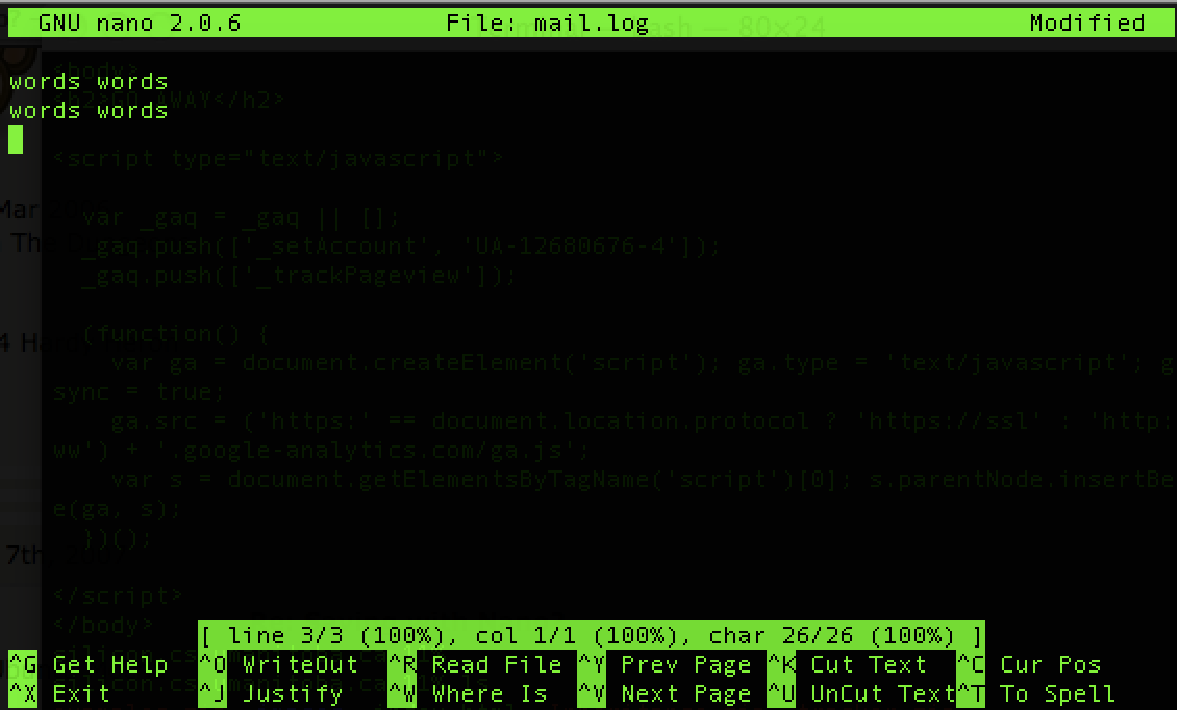
\includegraphics[scale=0.6]{shell/nano.pdf} 
		\caption{What nano looks like}
		\label{nano}
\end{figure}
you can see that nano has a list of available commands at the bottom of the screen.  
The caret (or hat or this thing: `\verb|^|') means `use the ctrl button'.
So, \verb|^|X means ctrl-x, which quits, asking if you want to save the `buffer' 
(that's your file) before you quit.

There are a few things not listed, like pressing F3 saves, F2 saves and quits. 
There's a multitude of functions to use, check out the surprisingly helpful
help section by pressing ctrl-g.

Though {\tt nano} and {\tt pico} are good, people will make fun of you 
if you don't know how to use {\tt vi(1)} or {\tt emacs}.  Check out the section
on {\tt vi} to learn how to use that.
% TODO - link to vi

 
 


\subsection{Searching}
I think we've all been in the situation that we either:
\begin{enumerate}
\item Forgot where something was
\item Don't know where we saved something
\item Accidentally moved something
\item Just flat out never knew where something was
\end{enumerate}

Luckily, the shell give us pretty good access to find the things we've lost, and even do a little better than just help us find it!

\subsubsection{The {\tt find} and {\tt locate} commands}
The simplest way to find files is by using the {\tt find(1)} command.  The {\tt find} 
command works best if you have a notion of where the file you're looking for might be. 
Using {\tt find} on the entire filesystem is not very efficient and tends to run into issues. 
There are many ways to use {\tt find}, but first we'll look at how to find files by name.

The basic way to use {\tt find} to find a file by name is as follows:
{\tt
\begin{verbatim}
find [whereToLook] [-name WhatToLookFor]
\end{verbatim}
}
The thing that makes the {\tt find} command both powerful and awkward
is that the user must specify where {\tt find} should start looking. In general
the places you might want to look might be the present working directory (`.'), the 
root of the filesystem (`/') or your home directory (`$\sim$'). Then the {\tt -name} 
parameter makes find look for a file that has the filename specified. 
 
{\tt
\begin{verbatim}
# pwd
/home/john/projects
# find . -name readme
./arduino/readme
./avr/readme
# find ~ -name readme
/home/john/projects/arduino/readme
/home/john/projects/avr/readme
# find /home/john/projects/avr/ -name readme
/home/john/projects/avr/readme
#
\end{verbatim}
}
One important thing to note is that the filename is case sensitive. If you have 
GNU find (which is not standard on all distributions), you can use {\tt -iname} 
in replacement of {\tt -name}.
{\tt
\begin{verbatim}
# find . -iname readme
./arduino/readme
./avr/readme
./perl/README
./python/Readme
#
\end{verbatim}
}
Notice how the various capitalizations of readme were found.

If you only know part of the filename, you can use a wildcard 
to find your file.  Say that you know that a file ends in `me', 
but don't know the rest of the filename, you could do this:
{\tt
\begin{verbatim}
# find . -name \*me
./arduino/readme
./avr/readme
./python/Readme
#
\end{verbatim}
}
Notice the \\ front of the *.  If you do not do that, the 
{\tt find} command will be looking for a * in the filename, 
which is not our intention.

Another thing that find can do is list every file starting in some 
directory.  To do this, just leave out the {\tt -name filename} 
and let it run. You'll probably not want to do this on a directory 
that has lots of files. This output isn't too useful, unless you 
pipe it to grep.

Another way to search is by using the {\tt locate(1)} command.  
{\tt locate} is not in the base installation of all operating 
systems, and requires some extra overhead due to the way 
it works.

{\tt locate} is a good search command since it is very fast.
{\tt locate} has some extra overhead in that it indexes the 
filesystem regularly to maintain a list of files and where they 
are. When {\tt locate} is run, it searches for the file in it's
database of files instead of the live filesystem. Though it's
blazingly fast, the data might be out of date. That is, if you've
changed things it will not immediately reflect the change.

The best thing about {\tt locate} is how easy it is to use.
{\tt \begin{verbatim}
# locate text.txt
/home/john/Library/TeXworks/completion/tw-context.txt
/home/john/4140/a2/MysteryPlaintext.txt
/home/john/4140/a2/plaintext.txt
/home/john/4140/aes/build/Debug/test1plaintext.txt
/home/john/4140/aes/build/Debug/test2plaintext.txt
/home/john/4140/aes/build/Debug/test3plaintext.txt
/home/john/projects/grep/text.txt
[snip]
#
\end{verbatim}
}

Running locate might be faster, but the results might be stale... while 
find will return reliable results slowly. To know how much faster locate is, look at the 
following results I got using a simple test.
{\tt \begin {verbatim}
# time find / -name text.txt
[snip]
real    4m58.989s
user    0m9.749s
sys     1m30.039s
# time locate  text.txt
[snip]
real    0m1.390s
user    0m0.916s
sys     0m0.100s
You have new mail in /var/mail/robg
\end{verbatim}
}
Locate took just over a second, while find took about 4 minutes. 


To sum things up, there is an obvious trade-off between reliable results and speed. But, 
{\tt find} has the feature to search a specific directory, which makes the search much faster 
and have reliable results. Both are useful tools and have their own uses, and you should 
choose the right tool for the job.

\subsubsection{Searching for text using {\tt grep}}
The {\tt grep(1)} command is a fantastic command that has 
many uses, though some of them are not immediately obvious.

Grep stands for  {\tt g}lobal {\tt r}egular {\tt e}xpression and
{\tt p}rint, which doesn't really define what it does very well. 
For people new to UNIX environments it doesn't seem too 
useful either, but is one of the most powerful tools available 
on the command line.

In UNIX, everything is a file.  In general, we want to look 
thought these files. We don't want to open each one and
search though it visually, or use a search in {\tt vi} for each 
file, so we'll use grep.

{\tt grep} takes input, which will inevitably be a file, which 
can (correctly or incorrectly)interpreted as text. {\tt grep} will take this
text and search for it in the input, returning the result in various requested
ways.

There is two ways to get input into {\tt grep}: piping or specifying files. 
If no files are specified to look through, then {\tt grep} will wait for {\tt stdin} for input.

Basic usage looks something like this:
{\tt \begin{verbatim}
# grep whatToLookFor [List] [of] [files] [to] [search] [though]
- or -
# cat file.txt | grep whatToLookFor
\end{verbatim}
}

Clearly {\tt cat} isn't the best option to send text to the pipe,
but it demonstrates how to use {\tt grep} with a pipe.


The best way to understand grep, is to see it in use. Say we have a text file named {\tt text.txt} that looks like this:
{\tt \begin{verbatim}
The quick brown
fox jumped over
the lazy dog.
Lorem ipsum dolor sit amet, consectetur adipisicing 
elit, sed do eiusmod tempor incididunt ut labore et 
dolore magna aliqua. Ut enim ad minim veniam, quis 
nostrud exercitation ullamco laboris nisi ut aliquip ex.
\end{verbatim}
}

So, let's try to grep for a few things, a few different ways. First, 
we'll look for the word `the' in the file.
{\tt \begin{verbatim}
# grep the text.txt 
the lazy dog.
#
\end{verbatim}
}
By default, {\tt grep} returns the whole line that the 
word you're searching for appears on. Also, notice that the {\tt grep} is 
case-sensitive by default. Let's try searching case insensitive, using
the {\tt -i} flag.

{\tt \begin{verbatim}
# grep -i the text.txt 
The quick brown
the lazy dog.
\end{verbatim}
}
Now the search has found both capitalizations of the word `the'.

Now, a more interesting case.  You're trying to find a function
you wrote.  All you know is which directory, part of the 
function name and that it has a .py suffix.

{\tt \begin{verbatim}
# grep printFile *.py
readTree.py:def printFile(name, depth):
readTree.py:            printFile(line[depth], depth)
#
\end{verbatim}
}
This command searches for the text `printFile' in all .py (* meaning `anything' and we said *.py) 
files in the current  directory. 

Now, what if we know a file is somewhere in some directory tree
(say some big program with lots of subfolders and files), but don't
know what it's called.  But, we do know some text in the file.
For this problem we'd use the {\tt -R} flag, which stands for recursive search.
A recursive searches in a folder, and any of it's subfolders, so it's exactly what we want.  
This flag will make grep look in all files and directories in the 
directory given.

{\tt \begin{verbatim}
# grep -R "Some known text" folderTreeToSearch
\end{verbatim}
}

% TODO - the _file_ matches, -v
% or should we... grep is getting kinda big anyay...

{\tt grep} is also good at searching through large files for text you 
are looking for.

Say that you have a .java file that has grown excessively large (as Java is known
to do).
There's method you know the name of, and you want to see all the references to it.

{\tt \begin{verbatim}
# grep -R myGreatMethodName BigJavaFile.java 
\end{verbatim}
}

And if we want to get the line numbers of the references, we can use the -n flag to return
the line numbers your text was found on.

One of the most useful functions of grep is the ability to use regular
expressions in it's search terms.
% TODO - Sean, can you do the regexing... I'm not so hot at it.

% TODO - pointer to look at the oreilly book on regexes - Sean, that's for you too.




% these are to help not break diff/patch/merging
% The heading roughly match that of the outline
% the sub-ing of the heading might be off.
\subsection {Process info}

So, we've discovered a lot about the tools available to us, and 
we've been running programs... but what if a program `goes wild'? And, 
how to we see what is running on the computer in the background?

Most of us have done this in Windows at one time or another. Windows
calls it Task Manager, and it looks something like figure~\ref{fig:Explorer-Applications}.
\begin{figure}[htbp]
	\centering
		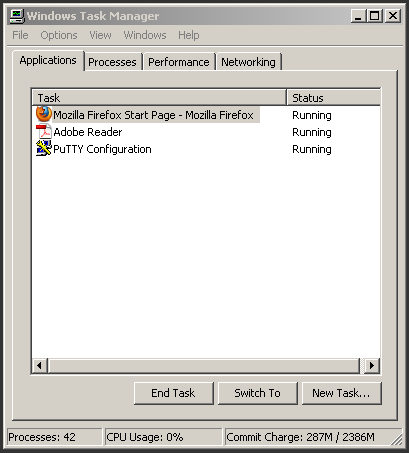
\includegraphics[height=3in]{shell/Explorer-Applications.png}
	\caption{Windows Task Manager, showing the running Applications}
	\label{fig:Explorer-Applications}
\end{figure}
From here you would usually kill any program that has gone wild
and is bringing down the machine or has stopped responding.

To get an idea of what the UNIX commands are showing us, you need
to look at the Processes tab of  Task Manager. Check out figure~\ref{fig:Explorer-Processes}.
\begin{figure}[htbp]
	\centering
		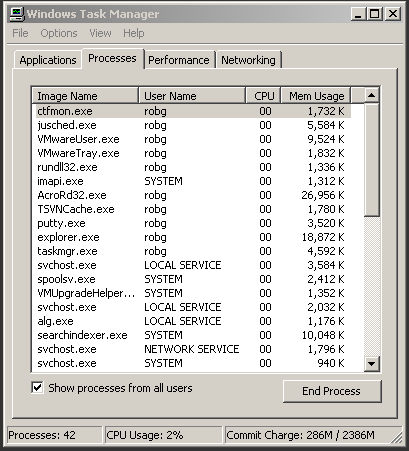
\includegraphics[height=3in]{shell/Explorer-Processes.png}
	\caption{Windows Task Manager showing all running processes.}
	\label{fig:Explorer-Processes}
\end{figure}
There's a lot of crap there that you didn't start as a program. There's a few
recognizable processes running... like AcroRd32 is probably Adobe Reader. And putty.exe
is most likely PuTTy running. But what is all this other junk? Well, they're daemons running in the
background making everything else work properly. 

Daemons are best defined as `queryable services'... something running 
in the background that is listening for some event to happen, and 
you can check on it's status if you so desire. If you have iTunes installed
you'll see iPod services, waiting for an iPod to be connected to the computer.

Now... to UNIX commands. Your tool to use here is {\tt ps(1)}, which stands for
{\tt p}rocess {\tt s}tatus. Waiver: ps has slightly different switches for different
operating systems. The commands listed are tested on OpenBSD and Debian.

{\tt \begin{verbatim}
# ps
  PID TT  STAT       TIME COMMAND
  1180 p0  Ss      0:00.01 -ksh (ksh)
 11063 p0  R+      0:00.00 ps
\end{verbatim}
}

Ok... so apparently I'm running ksh, which is Korn shell, and ..... ps.  {\tt ps} 
just told me I'm running ps. Great. Here's an example with more programs running.

% TODO - ugh openBSD gives kind of gross output (for newbs) - debian is a little cleaner.
{\tt \begin{verbatim}
# ps    
  PID TT  STAT       TIME COMMAND
 1180 p0  Is      0:00.01 -ksh (ksh)
 5255 p0  S+      0:00.01 screen
16749 p5  Is      0:00.01 /bin/ksh
  285 p5  I+      0:00.01 vi stuff.txt
16838 p6  Is      0:00.01 /bin/ksh
16094 p6  I+      0:00.01 less sent
27428 p7  Ss      0:00.01 -ksh (ksh)
 4765 p7  S+      0:00.01 less aFile
 1260 p8  Ss      0:00.01 -ksh (ksh)
10119 p8  R+      0:00.00 ps
# 
\end{verbatim}
}

We can see some important information about the processes. We can see
the PID, or process identifier. We'll use this later.

We can see which terminal it's running on. If you're connecting to the machine multiple times
with or have multiple terminal windows open, you'll have multiple terminals showing up here, each with it's own 
shell running (ksh, sh, bash, dash... whatever you use).

%TODO make sure this matches what's above... especially if you change what's above!
After that you see the command that is running.  This is program that is running, and like Windows
Task Manager's process tab, it's the ugly name for it... the actual program name that is running. The nice 
thing is that you can see the actual command that was called to launch the program. Above you can see {\tt vi stuff.txt}, 
which was the actual command to run vi on the file stuff.txt.

But... as naturally snoopy people... we'd like to know what other people are running.
For this we use the {\tt -a} or {\tt -A} flags. Another good flag is {\tt -x}, which 
removes the need for a terminal (read: a daemon process). I find that using {\tt ps -ax} 
does what I want on every machine I've worked with. It shows all processes from all users
and daemons and lists them for me. 

This list is a little unruly though. So, let's chop it down to what we want. 
We'll talk about piping later...
% todo - when is later
 for now just say that the output 
of one program can be the input to the next. So, we can pass the output of 
{\tt ps} to the input of {\tt grep}. Let's look for all the times that {\tt less}
is running.
{\begin{verbatim}
# ps -ax | grep less
16094 p6  I+      0:00.01 less sent
 4765 p7  I+      0:00.01 less aFile
# 
\end{verbatim}
}

Well, that works! But, people have done this so frequently that someone made a program
to do exactly this for us! Again, this is not standard. The program is called {\tt pgrep(1)},
which is literally `process grep'. It only returns the process id, which at first seems kind of useless,
but we'll find some good use for it. There are plenty of command-line switches to make it 
more useful for you too!

% sub sub sub section top?
Processes are always changing... it's nice to organize the processes in order 
of how much CPU time they are getting. Luckily most UNIX-like OSes have implemented a
tool to do this for us, lovingly named {\tt top(1)}.

%TODO - get a screenshot of this... on a machine that is NOT a server and is NOT running as root

There's a lot of information shown in a top screen. The key things to note is that
it automatically updates every second to stay recent. You can see the 
percentage of the CPU's time the top process is taking, the process ID, and who owns that process.
In short, it's everything you need to know!

There is a strange thing in the top left corner of the {\tt top} screen, called `load averages'.
It will look something like

{\tt load averages: 0.09, 0.10, 0.08}

This is the number of processes waiting to be run on the CPU over the last minute, last 5 minutes and last 15 minutes respectively.
This is a good indicator of how busy your computer has been over the last while. If this number is over 1 it means that your computer
can't keep up with the number of processes that are requesting to be run. This is common and nothing to be alarmed about. If the 
numbers go over 5, you'll start to notice the machine slowing down to requests. If the numbers go over 100 it's very
very bad, and you might not even be able to make {\tt ssh} connections to the machine any more.


% TODO - kill - Sean, this one's for you. talk about pgrep | xargs kill and the dangers therein, if you want!
			
\subsection {Other (screen, test....) }


\subsection	{Scheduling tasks  }
\label{subsection:cron}

Scheduling a task to run at regular intervals, or once some time in the future 
is quite simple in a UNIX environment.

\subsubsection{Regular Intervals}v
UNIX has a built-in service to run services at regular intervals, named {\tt cron(1)}
which (debatably) means `chronology'. {\tt cron} runs tasks on a schedule that is
defined in the user's {\tt crontab(1)}. The {\tt crontab} is a file with 
a specific layout that {\tt cron} reads to see when tasks should be run.

A crontab entry has 5 values, then the command that should be run. 
The  values are 
\begin{enumerate}
    \item the minute to run values (0-59)
    \item the hour to run values (0-23)
    \item the day of month to run (0-31)
    \item the month to run (1-12)
    \item the day of the week to run (0-7)
\end{enumerate}

\begin{verbatim}
*    *    *    *    *  command to be executed
┬    ┬    ┬    ┬    ┬
│    │    │    │    │
│    │    │    │    │
│    │    │    │    └───── day of week (0 or 7 are Sunday)
│    │    │    └────────── month
│    │    └─────────────── day of month
│    └──────────────────── hour
└───────────────────────── min
\end{verbatim}

If you want to run a command every hour, put a star in that spot {\tt *}.

So, here are a few examples of crontab entries:

\begin{verbatim}
30      1       *       *       *       /bin/sh /etc/daily
30      3       *       *       6       /bin/sh /etc/weekly
30      5       1       *       *       /bin/sh /etc/monthly
\end{verbatim}

The first one is daily, the 30th minute of 1am. The
minute and hours are specified, the rest have stars, meaning at 1:30am 
every day, every month, every day of week.

The second entry is is at 3:30 am on Saturday (the 6th day of the week).

And the third entry is at 5:30 am on the first day of the month. 

There are two important commands with {\tt cron}. The first one is{\tt crontab -l},
which will give you a {\tt l}isting of your crontab.  If you want to change your 
crontab, use {\tt crontab -e}, which will open your crontab for editing in your 
\$EDITOR (usually vi). If \$EDITOR is not set, there is another way to set your crontab.

\begin{verbatim}
#crontab -l > file.txt
\end{verbatim}

Then edit your crontab in file.txt. When you're done editing the crontab, set it as
your active crontab by using:

\begin{verbatim}
#crontab file.txt
\end{verbatim}

% TODO: talk about how standard out is emailed to the user

\subsubsection{Run once {\tt at(1)} a certain time}

The {\tt at(1)} command allows you to run a command (including running shell scripts) 
at a certain time. The at command differs from {\tt cron} on that it only 
runs the command once.

The {\tt at} command is very flexible for what it accepts as arguments,
but is a little strange in how it accepts the job. The most
common usage is:

\begin{verbatim}
at now + 3 minutes 
/run/this/task.sh    
[control-d]
\end{verbatim}

This  {\tt at} job will run in 3 minutes, and execute whatever is
in {\tt /run/this/task.sh}. The strange thing to notice is that I 
had to use a {\tt ctrl-d} to end the input. This is because 
{\tt at} expects input via standard in, and {\tt ctrl-d} marks the 
end of a file (or the end of input). Another, equivalent way of running this command would be

\begin{verbatim}
#echo /run/this/file.sh | at now + 3 minutes
\end{verbatim}

Which uses a pipe to send the command to {\tt at}'s standard in.

The units added to the date can be in minutes,
hours, days, weeks, months or years, which makes {\tt at} easy to work with. It's also 
possible to use a Month/day/year (formated MM/DD/YYYY) date with {\tt at} if you're not in 
the mood for addition.

If you want to see what jobs you've assigned to {\tt at}, use {\tt atq(1)}.
The jobs assigned to {\tt at} are added to a queue, so the command is 
read out `at queue', which is exactly what you'll be looking at when you 
run it.

And finally, if you want to remove an {\tt at} job, use {\tt atrm(1)}.
When you run {\tt atq} you'll see that the jobs are enumerated (have numbers before 
the dates). To remove a job run {\tt atrm 5}, replacing 5 with the job number you want to remove.
			
\subsection {Where to find stuff...} 
		

\subsection {Programs in UNIX}

	% introduce Magic numbers and the difference between a script and a binary 

	There are two types of programs you can run in an UNIX-like operating system.
	There are compiled files called binaries or executables and user-readable 
	files called scripts. For comparison, a binary is an .exe file on in Windows and a script 
	is loosely like a Windows batch file.

	There is a large difference in how these files are run by the operating system.
	Binaries are special files that are directly run by the operating system, while
	scripts are a list of commands that are run by a program (such as bash or 
	perl - but we'll get to that later!).

	Let's get into the details of these two types of files.

% http://en.wikipedia.org/wiki/Magic_number_%28programming%29

\subsubsection {Executables} 

	
	Executables are programs! They are run directly on the system, much like .exe programs
	in Windows. A binary is specific to the system it is running on, and it not very portable.
	A program that is compiled for 64 bit Red Hat Linux will not run on 32 bit OpenBSD, and vice versa.
	Some executables might be portable, but there is no guarantee that it will work. 
	
	So, we've called this a `binary file', now what does that mean. You probably know that 
	binary is just a bunch of {\tt 1}'s and {\tt 0}'s, and that's true for this too... but much
	more than that. A file being a binary means that a computer can run the commands natively. These
	commands are in binary form, hence, binary. If you want to know more about this, research `machine language'
	and `ELF executables'.
	% I totally want to say ELF format, but that says 'format format'.
	
	Overall, binary files are not human-readable. They are compiled programs that run natively on a particular machine
	architecture.

\subsubsection {Scripts}
	Scripts are user-readable and user-writable programs.  You can open any script using
	the text editor of your choice. Scripts are literally text files that contain commands
	that will be run by some program. UNIX-like operating systems have many different
	types of scripts that they can run `out of the box', though it varies which scripting 
	languages are available from distribution to distribution.
	
	Programs that `run' scripting languages are called `interpreters', taking and running 
	the commands given in a given script. Common interpreters are {\tt sh}, {\tt bash}, {\tt ksh},
	{\tt perl} and {\tt python}. Perl and Python are fully-featured programming languages that
	are very powerful and very flexible.  You might recognize {\tt sh} or {\tt bash} as programs you
	use when using the terminal... and you're right, they're one in the same. {\tt bash} and {\tt sh}
	scripts are commands you can run using the terminal, but grouped together to do a task for you.
	Let's take a look at an example {\tt bash} script, and the structure that is common to all scripts.
	
	{\begin{verbatim}
	#!/bin/bash
	echo Hello World!
	\end{verbatim}
	}
	
	In true programming form, that's our first bash script, and it's a hello world program!
	There's a number of lessons we can take away from this.
	
	Note the first line. the {\tt \#!} is important to all scripts, it's the line that tells the 
	system which interpreter to use. The {\tt \#!} is a special sequence, a magic number, that 
	tells the system that the file being run is a script. The text after the {\tt \#!} is executed, meaning 
	that you can put command-line switches after the call to the interpreter.
	
	After that, the script below is sent to the interpreter you requested. In the example above, we're calling
	{\tt bash}, which is a type of shell, and telling it to print out the text `Hello World'. If you're in
	a shell now, you can try to print something out using the {\tt echo} command - which literally echoes what you 
	send to it.
	
	One problem with scripting languages is that it is inherently slow. Instead of having a list 
	of commands to run on the processor, it's a list of commands to be read by an interpreter, which
	in turn makes commands that run on the processor. This extra step, interpreting the code, slows down processing time.
	That being said, it's still very fast. In an environment that speed is key, you should maybe consider a 
	language that creates compiled binary.
	
\subsubsection{The {\tt file} command}

	UNIX gives us a tool to determine what kind of file a file is, and it's called {\tt file}!

\begin{verbatim}	
#file program
program: Mach-O 64-bit executable x86_64
#file cCode.c
cCode.c: ASCII c program text
\end{verbatim}	

% TODO - tell how it works? Just give a teaser 'hey kids, check out ELF!', but we already did that.

\subsection {Permissions}
	% why 1777 is for idiots!
	
	Permissions are vital to the security of your information. The permissions to your files and folders
	determines who can, and who can not read your data. If these are set wrong, the wrong people can read
	your files... and chances are those people don't like you.
	
	The first thing to understand is are the permissions. Let's look at an {\tt ls -l} of a folder.
\begin{verbatim}
# ls -l
-rw-------   1 robg  staff  11705 18 Apr  2009 BachelorPartyList.ods
drwxr-xr-x   4 robg  staff    136 10 Jan  2011 Invoices
drwxr-xr-x   5 robg  staff    170 22 Dec  2009 LikelyUnimportantDocuments
-rw-r--r--   1 robg  staff  31575 29 Jun  2009 Picture.png
-rw-r--r--   1 robg  staff  53281 17 Dec  2009 Reservation.pdf
drwxr-xr-x  13 robg  staff    442 15 Dec  2009 Resume
-rwxrwxrwx   1 robg  staff  99868  3 Jan  2009 SlideShowV9.mov
-rw-r--r--   1 robg  staff   2928 22 Oct  2008 South_Park_Icon.jpg
-rwx--x--x   1 robg  staff    170 21 Oct  2011 swipe.py
\end{verbatim} 
We can see a small collection of files and folders here. The thing that we care about right 
now is the first column, which tells us this file's permissions. We can see sets of 
{\tt rwx}'s aver and over again. These literally translate to `read', `write' and `execute'. 
Those are pretty self-explanatory. They are repeated 3 times, for (in order) the owner of the file (robg),
the group assigned to the file (staff), and everybody (well, everybody else - not the owner or in the group).

So, our example, I don't want anyone else to see what's in BachelorPartyList.ods. Makes sense. Everyone else can 
read, but not change Picture.png. People can run, but not read the code of or change swipe.py. And finally, anyone can
read or change SlideShowV9.mov.

Permissions are (relatively) obvious with files... but not as obvious with folders. 
\begin{itemize}
	\item If a user has no permissions (does not have read, write or execute) they can not even {\tt cd} into the folder, and can not see the files in the folder.
	\item If a user has execute, they can {\tt cd} in to the folder, but not {\tt ls} the {\tt folder}
	\item If a user has write, they can add new files to the folder (even if they can't do an {\tt ls}).
	\item If a user has read, they can {\tt ls} the folder.
\end{itemize}
Note that even if a user don't have write on the folder, but has write on a file, the user can still change the contents of the file.

Now we have the basics of permissions... now to the commands
\subsubsection{{\tt chmod}}
	The {\tt chmod} command means `change mode'. Useful, right?... It really means `change permissions'.
	There's two ways to use the {\tt chmod} command to change permissions. The pretty way, and the good way.
	
	\textbf{The pretty way}: There's 3 different types of people we care about in the system: Owners, group and everyone.
	Let's make abbreviations for each of these: owners=o, group=g, everyone=a (all people).
	
	We already have abbreviations for our permissions: read=r, write=w, execute=x (because x is cooler than e).
	
	Now say that + means grant permission, and - means take away permission.
	
	So, the pretty way to give everyone read access to somefile.txt would be:
	\begin{verbatim}chmod a+r somefile.txt \end{verbatim}
	Which can be read literally as `change permissions for everyone, give read'.
	
	Or take away read from everyone, and group:
	\begin{verbatim}chmod ag-r somefile.txt \end{verbatim}
	Which is literally read `change permissions for everybody and group, remove read'.
		
	That's cool an all, but it's not exact, and is not used by people who are comfortable with permissions in UNIX.
	
	\textbf{The good way}
	We're going to use some pretty simple math to solve our problem. r=4, w=2, x=1. Those might look like 
	stupid numbers to choose initially, but they're actually kind of clever.
	
	It's actually derived from binary. Imagine a 3 bit binary number. If a user a r, the 1st bit is 1.
	If a user has write, the second bit is 1. If the user has execute, the 3rd bit is 1.
	
	This sounds needlessly complex... bear with me.
	
\begin{verbatim}
	perm   binary   decimal
	rwx -> 111   =  7
	rw- -> 110   =  6
	r-- -> 100
	
	--x -> 001   =  1
\end{verbatim}
For anyone that's seen binary numbers, this is a breeze. For those who haven't, it's non-trival.

Why is this way `better'? It's exact. Does a+x remove the other permissions from everyone? I don't know,
and it's harder to remember. Really, you don't need to do the math every time. In general, you only 
need to remember 7,6 and 1. They are by far the most common.

Now, putting it together. We write a 3 digit number. The first digit defines the 
permissions for the owner, the 2nd the group and the 3rd for everyone.

Give the owner all permissions, and nothing to everyone else
\begin{verbatim} chmod 700 somefile.txt \end{verbatim}
	

Give the owner all permissions, group read and nothing to everyone else
\begin{verbatim} chmod 740 somefile.txt \end{verbatim}	

Give everyone execute
\begin{verbatim} chmod 111 somefile.txt \end{verbatim}	
%todo: talk about how this could be done with \begin{verbatim} chmod 001 somefile.txt \end{verbatim}	?

\subsubsection{{\tt chgrp} and {\tt chown}}
We've seen the words `owner' and `group' tossed around a lot already. Here's what they 
actually mean.

Owner: usually the person that makes the file. The person that's `in charge' of the file. The user
is a user on the system, and there can only be one assigned to the file.

Group: usually ignored on a home computer, but on servers there are many of these. Daemons (tasks that run
in the background) should have their own group, at a university there would be a `students' group and a `faculty' group. 
Basically, who are you sharing this file with?

Everyone: Any user on the machine. A free-for all!

So, changing these: {\tt chown} is `change owner'. 
\begin{verbatim}chown robg someFile.txt \end{verbatim}
would make robg the owner of the file.

You can also add a group
\begin{verbatim}chown robg:awesomePeople someFile.txt \end{verbatim}
would make robg the owner of the file, and awesomePeople the group of the file.

And to just change the group:
\begin{verbatim}chgrp awesomePeople someFile.txt \end{verbatim}
	
If you're ever in doubt, try it... then do a {\tt ls -l} to see if you have your intended results.

\subsubsection{Why 1777 is for idiots}

If we ran the command {\tt chmod 777 somefile.txt}, it would give rwx to all users. In general, you don't
want to do that. What's this leading 1?

The 1 is called the `set uid bit'. It sets the user id of the person running the file (remember, it's executable) to the
user id of the owner. Basically, whoever runs the script, runs it with your permissions.

This has a lot of good uses. It's a good way to control access to some resource (configuration file, file repository) if you want
to be able to validate changes before letting anyone make changes willy-nilly. 

But, here's the catch.  1777 give whoever is running the script the same access you have (because of the set uid bit.), 
and anyone can edit the file (because everyone has rwx). So, you just let anyone run any command as you. If you're root 
and did this, I would edit the script to change your password, then take control of the system. 

Basically, making a file with the permissions 1777 lets anyone do anything as you on the system. 1711 probably is what you want,
I'll let you think about why.

\subsection {Piping}
Piping is one of the things that makes the UNIX terminal so powerful. Piping,
in general, is a way of changing the input to a program, or the output of a program.

What the heck does that mean? Try this:

\begin{verbatim}
# echo Some words
Some words
\end{verbatim}

The {\tt echo(1)} program echos what the user typed to `standard out' (or STDOUT as 
programmers often spell it), which 
gets printed onto your terminal. This is the default behaviour of a program's standard
out.
	
We can redirect the program's standard out to print to a file by using the greater
than sign {\tt >}. Think of {\tt >} as an arrow pointing out from the program to your file.

Check out this example. Remember that {\tt cat(1)} prints out the contents of a file for us.

\begin{verbatim}
#echo Donald Knuth > name.txt
#cat name.txt 
Donald Knuth
#
\end{verbatim}

So, we wrote the words Donald Knuth to a file, then printed out the contents of the
file... which returned Donald Knuth!

What if we do it again?
\begin{verbatim}
#echo Donald Knuth > name.txt
#cat name.txt 
Donald Knuth
#
\end{verbatim}

We only have one Donald Knuth, not two. This is because the {\tt >}	operator
will destroy the file before it prints to it. There is a different operator
to append... which is two greater than signs {\tt >>}.

\begin{verbatim}
#echo Donald Knuth >> name.txt
#cat name.txt
Donald Knuth
Donald Knuth
#
\end{verbatim}

The {\tt >>} operator is good for logging to a file, since it always appends
to the end of the file.

Piping can do one better than that, too. The output of one program can 
be piped to the input of another program. We do this by using the `bar' or 
`pipe' character on the keyboard {\tt |}. It's usually above the return key.

\begin{verbatim}
#ls
name.txt
#touch muzak.mp3 daemon.txt exams.txt
#ls
daemon.txt	exams.txt	muzak.mp3	name.txt
#ls | grep mp3
muzak.mp3
#
\end{verbatim}

In the example, we do an {\tt ls(1)} that shows us all the files in the directory,
then we pipe {\tt ls} to {\tt grep}, which lets us filter the results that were 
output by {\tt ls} down to the results we want to look at. The results of the 
grep are then put onto the terminal. 

Using pipes, we can even use grep multiple times to filter results to 
exactly what we want.

\begin{verbatim}
# grep named /var/log/messages | grep starting | grep "Nov 29" 
Nov 29 20:44:32 path named[29612]: starting BIND 9.4.2-P2
\end{verbatim}

This is useful for searching through log files that
have lots of entries in them.

It is also possible to redirect input from the command line, using the
less than sign {\tt < }

\begin{verbatim}
#cat < name.txt 
Donald Knuth
Donald Knuth
\end{verbatim}

The {\tt <} sign will take the contents of a file, and 
pass them as if they were piped to the program you 
have piped it to. In the example, the contents of name.txt
are piped to {\tt cat} to be printed out. There is not 
a lot of times this is used, but can be useful.

% Yes, I left out the << redirection. It's not super useful, imho. -rg

Programs have more than one way of printing output!
Standard out is for the normal output of a program, but what about 
output that is not normal, such as error messages? These are printed 
out to standard error (or STDERR). This output can also be redirected
using the {\tt 2>} marker.

TODO example. 

The most frequent use for redirecting standard out is to 
keep cron jobs silent. If a program that is running as a cron job
has any output, that output is sent via email to the user that
owns the cron job. To keep cron jobs silent, some people redirect the 
output to {\tt /dev/null}, which is a device that does nothing with the output (and isn't really a device!).

An example of a cron job that redirects both standard out and standard error would look like this:

\begin{verbatim}
30 5 1 * * /root/doBackup.sh >/dev/null 2>/dev/null
\end{verbatim}    

This is nice, since the cron task will never try to send you an email, 
but this also means that the cron job will not tell you if it's not working properly!

\subsubsection{What is 2\textgreater\&1?}
This is a weird one, and deserves it's own subsection (so it shows up in the 
table of contents).

There are two special variables available on the command line, \&1
which is a variable that means standard out, and \&2 which is 
a variable for standard error. 

So this means that the standard error of the program should be 
piped to standard out, so it will all show up in one place!

One use of this syntax is to make a program have \underline{no} output
whatsoever. This is done for various reasons... and often is not the
right thing to do.

First, how it's done:

\begin{verbatim}
/root/bin/do_backup.sh >/dev/null 2>&1
\end{verbatim}

What is this doing?!?!

\begin{itemize}
\item runs the script `{\tt do\_backup.sh}' which is in `/root/bin'
\item pipes standard out to /dev/null. This means the output is throw away!
\item then, standard error is sent to the same file as standard out. Standard
out is being thrown away, so standard error is being thrown away with it.
\end{itemize}

This is a more common idiom than you may expect. This is frequently used in
cron jobs. The standard out is emailed to the user that owns the cron
job(see~\ref{subsection:cron} for more on that), and some people find this
annoying. A better solution is to have scripts only output errors do \underline{do}
want to see, to prevent valuable output to be lost to `/dev/null'.

\subsection {Help... {\tt man(1)}}
You've seen us using weird notation for UNIX commands. This is a (almost) standard
way of directing someone to the help files that exist on all UNIX systems. 
To get detailed help about how to use a program, or what configuration
options are available for a configuration file, use {\tt man(1)} (short for manual).

To get help on how to use help.. type {\tt man man}, which will 
tell you how {\tt man} works, where the files are stored, and 
command-line options on how to use it.

There are different sections that can be viewed for different commands.
Here is the list of the various sections available to be viewed:

\begin{itemize}
\item Section 1
user commands 
\item Section 2
system calls 
\item Section 3
library functions 
\item Section 4
special files 
\item Section 5
file formats 
\item Section 6
games (introduction)
\item Section 7
conventions and miscellany (introduction)
\item Section 8
administration and privileged commands (introduction)
\item Section L
math library functions
\item Section N
tcl functions
\end{itemize}

These can vary from system to system, but these are the usual sections available.

As you can see, there is many different types of help. To see the programming interface for 
built-in C functions, you would use man 3.

\begin{verbatim}
man 3 printf    
\end{verbatim}

This will tell you what to import to use the library function, and how it 
can be used.

If you don't supply a section number, your system will either default to the first one it files (starting a section 1), or {\tt cat}
all of the man pages together.

A nice trick that not everyone knows, is that system configuration files 
often have their own man page. {\tt man rc.conf} (which will bring you to {\tt man 8 rc.conf})will tell you 
how to use your rc.conf file (if you have one) and how to add items to start at boot time, versus {\tt man rc}
which will tell you how your system boots up.


\subsection {Making backups...} 

\begin{verbatim}
/usr/local/bin/mysqldump -u backup_user -A > /tmp/database.sql
FILENAME=database_`date +%Y%m%d-%H%M%S`.tar
tar czvf /tmp/$FILENAME /tmp/database.sql /usr/local/www/

/usr/bin/scp   /tmp/$FILENAME robg@parkway:/Users/robg/Archive/servername/

rm /tmp/$FILENAME
\end{verbatim}
% TODO: iterate on this later? Talk about how to use mktemp so it 
% doesn't wipe out file.

This can be automated by using crontab (see~\ref{subsection:cron}) and
using preshared keys(see~\ref{subsection:sshkeys}). Doing this will
run this script which,

\begin{enumerate}
  \item dump the database to a flat file
  \item tar up that file along with other folders you have selected
  \item move that tar file to a remote server
  \item remove the generated file
\end{enumerate}
  

\subsection {{\tt ssh} magic}

A short history: Since the beginning of time (the 1970s in UNIX time) there have been ways
to connect to computers that are not in front of you. This is pretty commonplace in our world, 
since that's pretty much what you do every time you view a website. But it hasn't 
always been that simple.

Say we want to have a shell on the remote computer we are connecting to. The easiest way 
to to this is to take the ascii character we are typing, and send that directly to the other
computer. Simple, right? But what about privacy. Doing this over the internet is like talking
about what you're doing REALLY LOUDLY in a room. What about your password? It'd be sent over the 
internet in a way that everyone can read it. Not ideal. 

The first remote shells did exactly this. Everything typed was sent in plain text across a wire to 
the remote computer. A program that does this is even installed on your computer right now! It' s
called {\tt telnet}, and it implements a very simple remote shell (and can do some other things).

Clearly sending plain text is not acceptable for passwords. In the old days, computers we're
really fast enough to encrypt and decrypt messages that are being sent across the internet,
but now they are! The best remote shell solution is called {\tt ssh(1)} (secure shell) and it's 
the standard way of using a remote shell. All the traffic created using ssh is encrypted so only the 
sender and receiver can understand
the messages. 

It's also quite easy to use. If your username is the same on both of the machines:

\begin{verbatim}
# ssh machine.unix.com
\end{verbatim}    

You can plainly see that the machine we are ssh-ing into looks like url. This is 
actually the hostname of the machine, and the world wide web (http) uses the same
notation to find the computer that you want a webpage from.

Sometimes your username can be different on the two machines, in this case:

\begin{verbatim}
# ssh username@machine.unix.com 
\end{verbatim}

This will tell the foreign machine that you are `username', and then will
match your credentials accordingly. 

The shell that you are given is exactly the same as the one that is on your local 
machine, but all the commands that are being run are being run 
remotely on the remote machine.

To exit out of the remote machine, type {\tt exit}, and you will be returned 
to your local machine.  

\subsection{Not typing passwords via authorized\textunderscore keys}
\label{subsection:sshkeys}
Don't like typing passwords? Like being rewarded for being lazy? Then this 
is something you'll like.

To set up a pre-authorized key, you'll need a private and public key pair.

To do this, use {\tt ssh-keygen}:

\begin{verbatim}
ssh-keygen -t rsa -b 2048
\end{verbatim}

The command uses -t for type (rsa 
is the current standard), and -b for how 
many bits the key should be (use a power of two, and nothing too small).

{\tt ssh-keygen} will prompt you for a few things, such as where to put the
keys it generates (the default place is good [~/.ssh/]), and for a password.
You should give it a password (which will encrypt your private key), but don't need to. 
The risk you run by not encrypting your private key, is that anyone who has it
can be you. As always, {\tt man ssh-keygen} is the best source for how the
program will run on your installation.

Go to your the .ssh directory in your home folder (~/.ssh/), you should see at 
least 2 files: id\textunderscore rsa, and id\textunderscore rsa.pub. These are your public and private keys
that will be used to identify you.  Open the file that has your public key (id\textunderscore rsa.pub)
in a text editor, and copy the contents.

The second step to set up authorized keys is to {\tt ssh} into the remote machine.
On the remote machine, go to (or create the folder if it doesn't exist) .ssh 
in your home folder (~/.ssh). In .ssh, open or create the file `authorized\textunderscore keys'
in your favourite text editor.
Paste the contents of the id\textunderscore rsa.pub file you copied from your computer.

Log out ({\tt exit}) and {\tt ssh} back in. You didn't have to type a password, and
if you did it was for your private key, and therefore your password wasn't blasted
over the internet!

\subsection{The differences between shells (a short, incomplete history)}
% bash is not sh
The first shell that was introduced was {\tt sh}, and introduced eariest versions of UNIX.
It is commonly called the "Bourne shell", named after the developer of the shell.
Even in the earilest versions, it introduced piping, if statements and other control blocks.
All current shells have used this for inspiration, and are frequently backwards-compatible to
 {\tt sh}.
 % do we need references for this? I stole it from wikipedia. I'm not an authority on this stuff -rg

Some shells use tab-completion to finish commands for users, other use the escape key,
and some don't don completion for us at all! You'll have to find the shell that works
for you and your preferneces. Some people have a prefernce for using as a hands-on shell, and
a different shell for scripting.

 Modern shells add user-friendly features, or allow for easier scripting. There are frequently
 minute differences that make the modern shells not compatible with each other.

 Overall, be careful when taking advice about a command from sources on the internet,
 as they might be for a different shell! It might not work at all with the shell you've chosen. Some might
 be compatible one-way, but not the other. Things that work in \tt{sh} should work in \tt{bash}, but
 things that work in \tt{bash} might not work in \tt{sh}. That's because \tt{bash} is backwards-compatible
 to \tt{sh}, but \tt{sh} is not forwards-compatible to the features added in \tt{bash}!

 \subsubsection{csh}
 The \tt{csh} shell is a bit of an old-school shell by today's standards, with some
 pundits defending it tooth-and-nail. It has been significant in the development of
 shells, introducing the \tt{~} notation as a shorthand way of creating paths
 to your home folder. The tilde notation is now used by most shells, as the tilde
has proven to be very useful.

\subsubsection{Korn Shell}
The Korn shell, or \tt{ksh}, was very popular for usage and scripting in the 1990s.
Some still use it as their daily shell, and maintains a strong following. There
are many daily batch jobs that rely on \tt{ksh} to run them to this day. It is known
to be highly reliable, and well-supported.

\subsubsection{bash}

The evolution of \tt{sh} is the Bourne again shell, or \tt{bash}. The name
is a play on words about the religious phrase of being "born again" - which
is clever.

As stated, \tt{bash} is backwards-compatible with \tt{sh}, allowing us to run
all \tt{sh} scripts. Shell scripting has largely moved to \tt{bash}/\tt{sh} scripts in the
recent history, with \tt{ksh} being used less frequency for new scripts.

This is the shell that ships with most Unix-like operating systems. This includes Mac OS,
and Ubuntu.
% though, they used to use dash... this is currently true
The \tt{bash} shell is so pervasive, that \tt{/bin/sh} often actually
starts up a \tt{bash} shell!




